
\section{\LTLtri Monitor}
\begin{frame}{3-Valued \LTL (\LTLtri) [Bauer, Leucker, Schallhart 11] }

3-valued \LTL evaluates \LTL formulas for finite words with an 
eye on \Def{possible future extensions}.

\ \\

%\pause

\begin{block}{Three Truth Values}
 
The set of truth values is \Def{$\mathbb{B}_3=\{\top,\bot, ?\}$}, where

\begin{itemize}

%\pause

 \item \Def{$\top$:} the formula is \Def{permanently satisfied} no matter 
how the current execution extends,

%\pause

\item \Def{$\bot$:} the formula is \Def{permanently violated} no matter 
how the current execution extends

%\pause

\item \Def{?:} denotes an unknown verdict; i.e., there exist extensions that can 
falsify or make true the formula.
\end{itemize}

\end{block}

\end{frame}

% ----------------------------------------------------------------------------



\begin{frame}{3-Valued \LTL}

\ \\

\begin{block}{\LTLtri Semantics}
Let $u \in \alphabet^{*}$ be a finite word. The truth value of an \LTLtri 
formula $\varphi$ with respect to $u$, denoted by $[u \models_3 \varphi]$, is 
defined as follows:

 \begin{equation*}
 	\left[ u \models_3 \varphi \right] = 
 		\begin{cases} \top & \text{if }~~~~~\forall w \in 
\alphabet^\omega : 
uw \models \varphi\\
 		\bot & \text{if }~~~~~\forall w \in \alphabet^\omega : uw \not 
\models \varphi\\
 		? & \text{otherwise}.
 	\end{cases}
 \end{equation*}
 
\end{block}

\end{frame}

% ----------------------------------------------------------------------------





\begin{frame}{3-Valued \LTL}

\begin{block}{\LTLtri Monitor}
 
Let $\varphi$ be an \LTL formula. The \Def{\LTLtri monitor} of $\varphi$ 
is the unique deterministic finite state machine $\monitor^{\varphi}_3 = 
(\alphabet, Q, q_0, \delta, \lambda)$, where $Q$ is a set of states, $q_0$ is 
the initial state, $\delta \subseteq Q \times \alphabet \times Q$ is the 
transition relation, and $\lambda: Q \rightarrow \mathbb{B}_3$, is a function 
such that:
\begin{equation*}
\lambda(\delta(q_0, u)) = \left[u \models_3 \varphi\right]
 \end{equation*} 
for every finite word $u \in \alphabet^*$. \qed

\end{block}

%\pause

\begin{example}{\LTLtri monitor for $a \, \U \, b$}

\vspace{-7mm}
 \begin{figure}
 \centering
 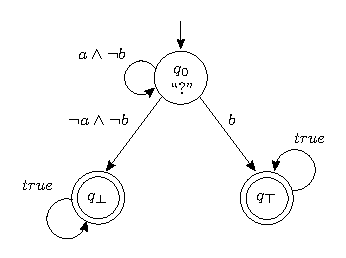
\includegraphics[scale=.85]{figures/exprop}
 \end{figure}

\end{example}

\end{frame}









\iffalse

\begin{frame}{\LTLtri}

\begin{example}

%\pause

\begin{tikzpicture}[->,>=stealth',shorten >=1pt,auto,node distance=2cm,
                    semithick]
 \tikzstyle{every state}=[draw=blue!75,fill=blue!10,minimum size=7mm]

\hspace{-1cm} $[u \models_3 \X p] = \top$ \hspace{1.5cm}
  \node[initial,initial text={}, state] (A) {};
  \node[state]         (B) [right of=A] {$p$};
  \node[state]         (C) [right of=B] {};
  \node[state]         (D) [right of=C] {};

  \path (A) edge node {} (B)
        (B) edge node {} (C)
        (C) edge node {} (D);
        
\end{tikzpicture}

%\pause

\vspace{.5cm}
\begin{tikzpicture}[->,>=stealth',shorten >=1pt,auto,node distance=2cm,
                    semithick]
 \tikzstyle{every state}=[draw=blue!75,fill=blue!10,minimum size=7mm]

\hspace{-1cm}  $[u \models_3 p \, \U \, q] = ?$ \hspace{1.2cm}

  \node[initial,initial text={}, state] (A) {$p$};
  \node[state]         (B) [right of=A] {$p$};
  \node[state]         (C) [right of=B] {$p$};
  \node[state]         (D) [right of=C] {$p$};

  \path (A) edge node {} (B)
        (B) edge node {} (C)
        (C) edge node {} (D);
        
\end{tikzpicture}

%\pause

\vspace{.5cm}

 \begin{tikzpicture}[->,>=stealth',shorten >=1pt,auto,node distance=2cm,
                    semithick]
 \tikzstyle{every state}=[draw=blue!75,fill=blue!10,minimum size=7mm]

\hspace{-1cm} $[u \models_F \F p] = \top$ \hspace{1.5cm}

  \node[initial,initial text={}, state] (A) {};
  \node[state]         (B) [right of=A] {};
  \node[state]         (C) [right of=B] {$p$};
  \node[state]         (D) [right of=C] {};

  \path (A) edge node {} (B)
        (B) edge node {} (C)
        (C) edge node {} (D);
        
\end{tikzpicture}

%\pause

\vspace{.5cm}

\begin{tikzpicture}[->,>=stealth',shorten >=1pt,auto,node distance=2cm,
                    semithick]
 \tikzstyle{every state}=[draw=blue!75,fill=blue!10,minimum size=7mm]

 \hspace{-1cm} $[u \models_F \G p] = \bot $ \hspace{1.5cm}

  \node[initial,initial text={}, state] (A) {$p$};
  \node[state]         (B) [right of=A] {$p$};
  \node[state]         (C) [right of=B] {$\neg p$};
  \node[state]         (D) [right of=C] {};

  \path (A) edge node {} (B)
        (B) edge node {} (C)
        (C) edge node {} (D);
        
\end{tikzpicture}
\end{example}
\end{frame}
\fi
% ----------------------------------------------------------------------------




% ----------------------------------------------------------------------------


\iffalse

\section{\LTLtri Monitor}
\begin{frame}{\LTLtri Monitor}

\begin{block}{3-Valued \LTL}

\begin{itemize}

\item The 3-valued semantics of \LTL (denoted \LTLtri) evaluates \LTL 
formulas for finite traces with an eye on possible future extensions. 
\item In \LTLtri, the set of truth values is $\mathbb{B}_3=\{\top,\bot, ?\}$
\end{itemize}

\end{block}

 \begin{block}{Example ($\varphi = a \, \U \, b$)}
  \begin{figure}
\centering
\begin{tikzpicture}[->,>=stealth',shorten >=1pt,auto,node distance=2.8cm, 
semithick, scale=.6, initial text={}, font=\small]
\node[state, accepting] (A)                    {$q_\bot$};
  \node[initial,state]         (B) [above right of=A] {$q_0$};
  \node[state, accepting]         (C) [below right of=B] {$q_\top$};
   
 \path  (B) edge [loop above] node  {$a \wedge \neg b$} (B)
        (B) edge node [left, yshift=2mm] {$\neg a \wedge \neg b$} (A)
        (B) edge node [right, yshift=2mm] {$b$} (C)
        (A) edge [loop below] node  {$\mathit{true}$} (A)
        (C) edge [loop below] node  {$\mathit{true}$} (C);
\end{tikzpicture}

\end{figure}
 \end{block}


\end{frame}
\fi

